\documentclass[a4paper,12]{article}
\usepackage{amsmath, amsfonts, amssymb, amsthm, bm, graphics, bbm, color}
\usepackage{graphicx}
\usepackage{subfigure}
\usepackage{mathtools}
\usepackage[table]{xcolor}
\usepackage{url}
\usepackage{mathabx}
\usepackage{cancel}

\usepackage{multicol}
\usepackage{float}
\usepackage{caption}
\usepackage{mathalfa}
\usepackage{hyperref}
\usepackage{afterpage}
\usepackage{multirow}
\usepackage[section]{placeins}

\captionsetup{font=footnotesize}
\captionsetup{width=\textwidth}
\DeclareMathAlphabet\mathbfcal{OMS}{cmsy}{b}{n}
\newtheorem{theorem}{Theorem}[section]
\newtheorem{lemma}[theorem]{Lemma}
\newtheorem{corollary}[theorem]{Corollary}
\newtheorem{proposition}[theorem]{Proposition}
\theoremstyle{definition}
\newtheorem{definition}[theorem]{Definition}
\newtheorem{example}[theorem]{Example}
\newtheorem{remark}[theorem]{Remark}


%center table entries
\newcolumntype{P}[1]{>{\centering\arraybackslash}p{#1}}


\newcommand\y{\cellcolor{gray!50}}

\newcommand\p{\cellcolor{gray!25}}

\makeatletter
\newcommand\makebig[2]{%
  \@xp\newcommand\@xp*\csname#1\endcsname{\bBigg@{#2}}%
  \@xp\newcommand\@xp*\csname#1l\endcsname{\@xp\mathopen\csname#1\endcsname}%
  \@xp\newcommand\@xp*\csname#1r\endcsname{\@xp\mathclose\csname#1\endcsname}%
}
\makeatother

\makebig{biggg} {3.0}
\makebig{Biggg} {3.5}
\makebig{bigggg}{4.0}
\makebig{Bigggg}{4.5}
\makebig{biggggg}{5.0}
\makebig{Biggggg}{5.5}
\makebig{bigggggg}{6.0}
\makebig{Bigggggg}{6.5}

\newcommand\bovermat[2]{%
    \makebox[0pt][l]{$\smash{\overbrace{\phantom{%
                    \begin{matrix}#2\end{matrix}}}^{\text{#1}}}$}#2}

\newcommand\bundermat[2]{%
    \makebox[0pt][l]{$\smash{\underbrace{\phantom{%
                    \begin{matrix}#2\end{matrix}}}_{\text{#1}}}$}#2}

\newcommand\partialphantom{\vphantom{\frac{\partial e_{P,M}}{\partial w_{1,1}}}}


\newcommand{\raisesym}[2]{\raisebox{0.5\depth}{$#1\Biggggg \}$}}

% redefine paper size
\setlength{\oddsidemargin}{0in}
\setlength{\textwidth}{6.4in}
\setlength{\topmargin}{-0.5in}
\setlength{\textheight}{9.9in}
\setlength{\headheight}{0in}

%slanted vector symbols
\renewcommand{\vec}[1]{\mbox{\boldmath$#1$}}
\newcommand{\vect}[1]{\boldsymbol{#1}}

%vertical d symbol for integrals
\newcommand{\dif}{\mathrm{d}}
\newcommand{\im}{\mathrm{i}}

\newcommand{\bbR}{\mathbb{R}}
\newcommand{\tr}{\mathrm{tr}}

\newcommand{\vvtheta}{{\bm {\vartheta}}}
\newcommand{\vvphi}{{\bm {\varphi}}}
\newcommand{\vtheta}{{\bm {\theta}}}


\DeclareMathOperator*{\esssup}{ess \, sup}

\begin{document}
\title{Angle measures for an MPT characterisation of a computed toy gun}
%\author{P.D. Ledger}
\date{5th April 2024}
\maketitle

Barrel has $\sigma_* = 1.45\times 10^6$ S/m and $\mu_r$ is varied ($\mu_r=100$ corresponds to carbon steel) and the receiver has $4.5 \times 10^6$ S/m and $\mu_r=1$ and is a stainless steel.  The barrel is hollow with a cap at one end.  The length of the barrel is 0.2 m, outer and inner radii of the barrel are 0.02 m and 0.01m, respectively. The box representing the receiver is 0.08 m $\times$ 0.01 m $\times$ 0.15 m.  A mesh of 21,132 unstructured tetrahedra, 5,525 prisms and elements of order $p=0,1,2,3,4,5$ are considered. The prisms are chosen to be used as boundary layers in the barrel, which has a smaller skin depth. 

\begin{figure}[h]
\begin{center}
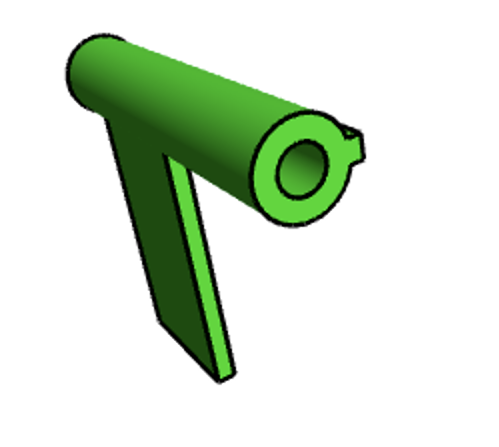
\includegraphics[width=0.5\textwidth]{Gun_modelv2_nonsym_StainSt.png}
\end{center}
\caption{Illustration of the toy gun. Barrel has $\sigma_* = 1.45\times 10^6$ S/m and $\mu_r$ is varied ($\mu_r=100$ corresponds to carbon steel) and the receiver has $4.5 \times 10^6$ S/m and $\mu_r$ and is a non-magnetic stainless steel.}
\end{figure}

When the eigenvalue curves  cross each other then this indicates the presence of eigenvalues with algebraic multiplicity greater than one.  The associated eigenvectors for an eigenvalue with algebraic multiplicity two 
 can be arbitrarily chosen as any two vectors that form a basis for the two-dimensional eigenspace.  In numerical computations, the computation of eigenvectors associated with eigenvalues $\lambda_n , \lambda_m$ is problematic when $\lambda_n \to \lambda_m$. 

 Angles between the computed eigenvectors using the metrics $d_R$ and $d_F$ are considered and  the approximations $d_E$ and $d_C$ that do not require knowledge of the eigenvectors. Notice the smooth transition of   $d_R$ and $d_F$ in the regions where the eigenvalues are repeated  and the associated {\bf peaks}.
While we know there are issues with the eigenvectors of repeated eigenvalues, the peaks are interesting as there is a {\bf smooth transition to them}.
  While $d_E$ and $d_C$ do not capture the peaks well, particularly $d_E$,  the normalising constant involved in the computation do identify the peaks.
  
  Note that $d_E$ and $d_C$ do capture the behaviour of $d_R$ and $d_F$ well for other objects when there are no peaks.



\clearpage
{}
\subsection{Barrel with $\mu_r=20$}

\begin{figure}[h]
\begin{center}
$\begin{array}{ccc}
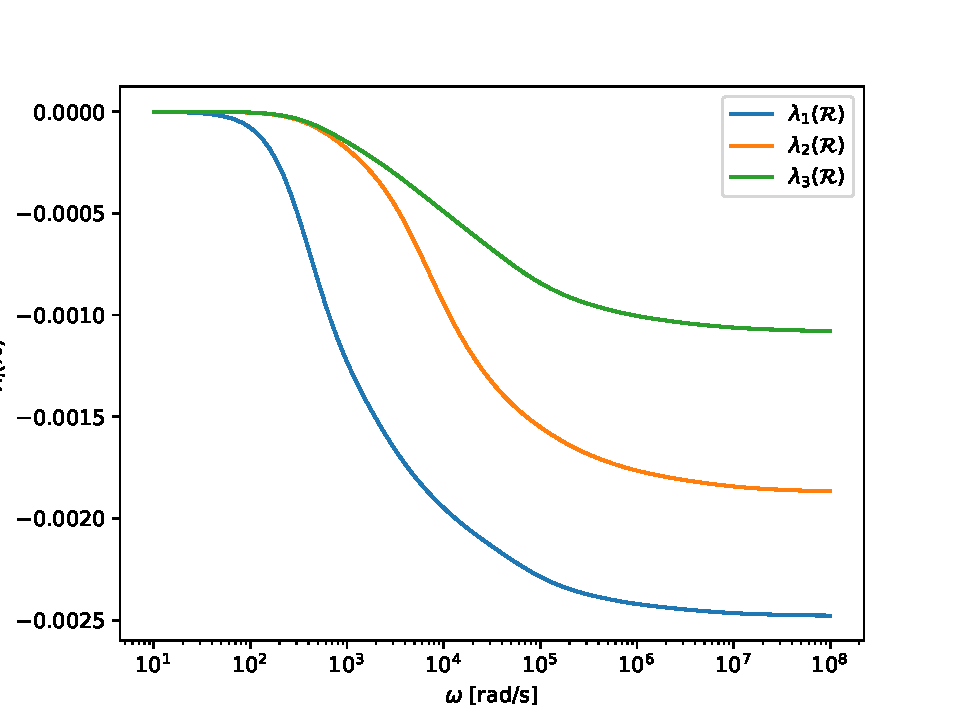
\includegraphics[width=0.3\textwidth]{mu20/OCC_Gun_modelv2_nonsym_StainSt_eig_R_al_0.01_20,1_sig_1e6,1e8_ord_5.pdf} &
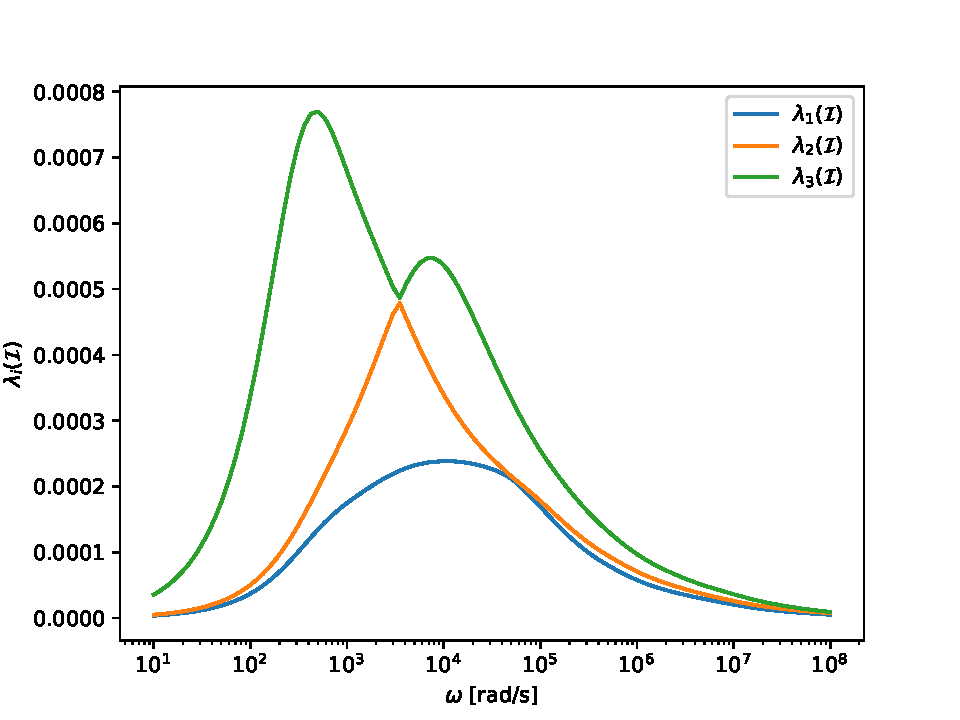
\includegraphics[width=0.3\textwidth]{mu20/OCC_Gun_modelv2_nonsym_StainSt_eig_I_al_0.01_20,1_sig_1e6,1e8_ord_5.pdf} &
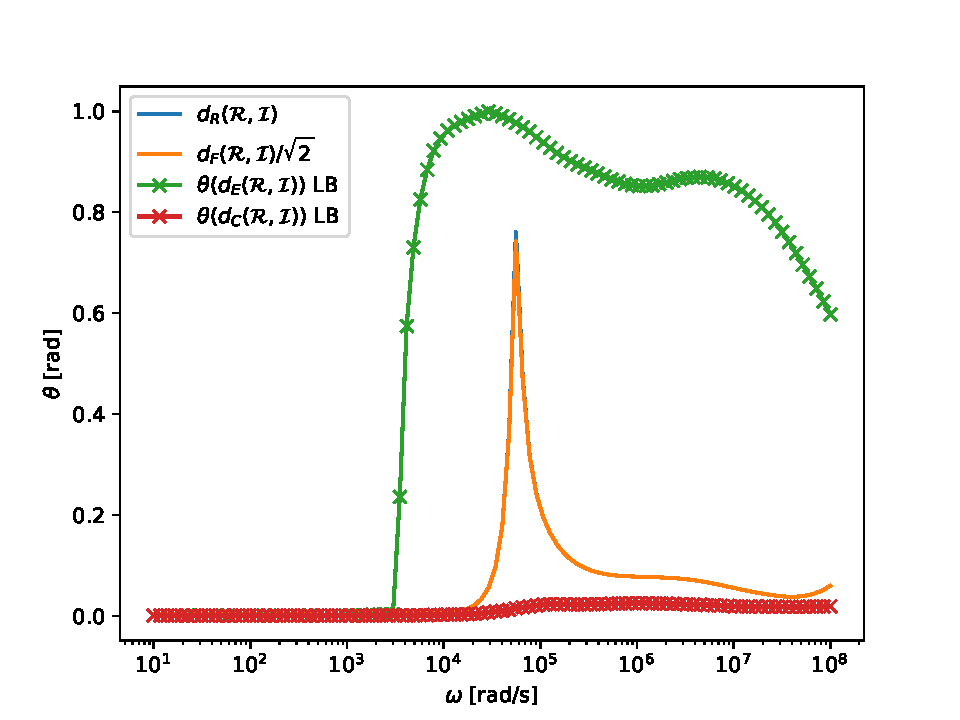
\includegraphics[width=0.3\textwidth]{mu20/OCC_Gun_modelv2_nonsym_StainSt_RI_al_0.01_20,1_sig_1e6,1e8_ord_4.pdf} \\
\lambda_i({\mathcal R}) &\lambda_i({\mathcal I}) &\text{Angles} \\ 
\end{array}$
\end{center}
\caption{Toy gun with $\mu_r=20$ in the barrel.  }
\end{figure}


\subsection{Barrel with $\mu_r=40$}

\begin{figure}[h]
\begin{center}
$\begin{array}{ccc}
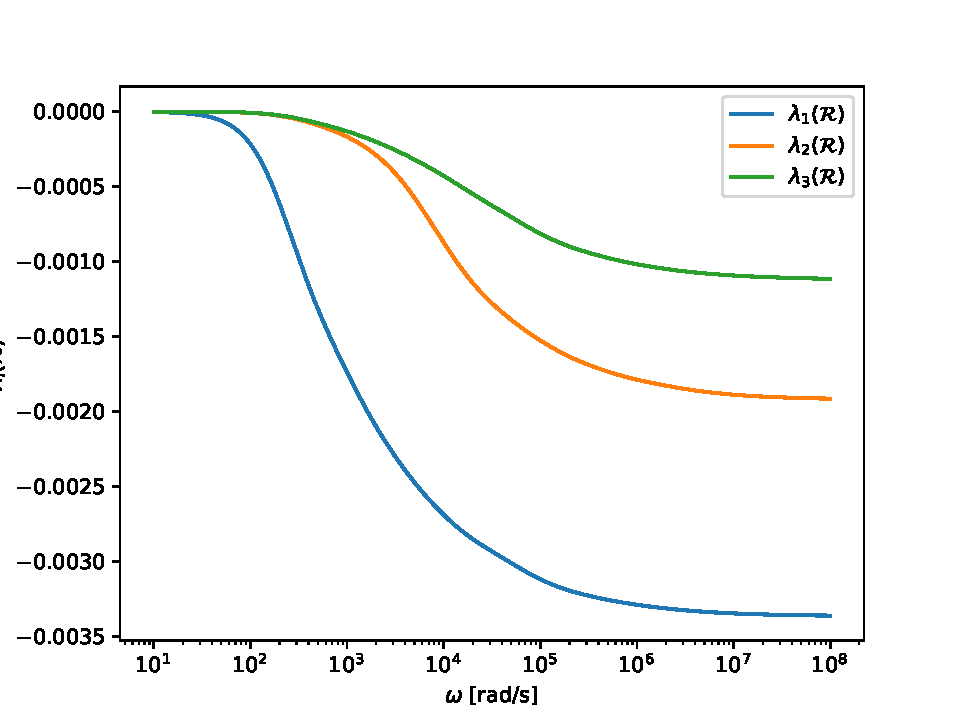
\includegraphics[width=0.3\textwidth]{mu40/OCC_Gun_modelv2_nonsym_StainSt_eig_R_al_0.01_40,1_sig_1e6,1e8_ord_4.pdf} &
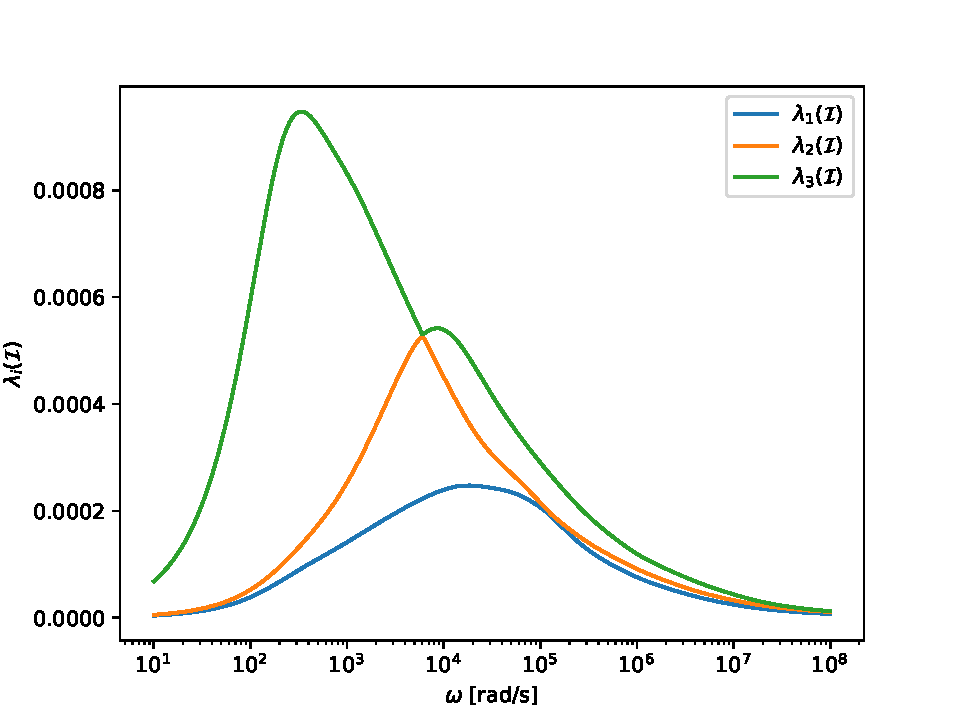
\includegraphics[width=0.3\textwidth]{mu40/OCC_Gun_modelv2_nonsym_StainSt_eig_I_al_0.01_40,1_sig_1e6,1e8_ord_4.pdf} &
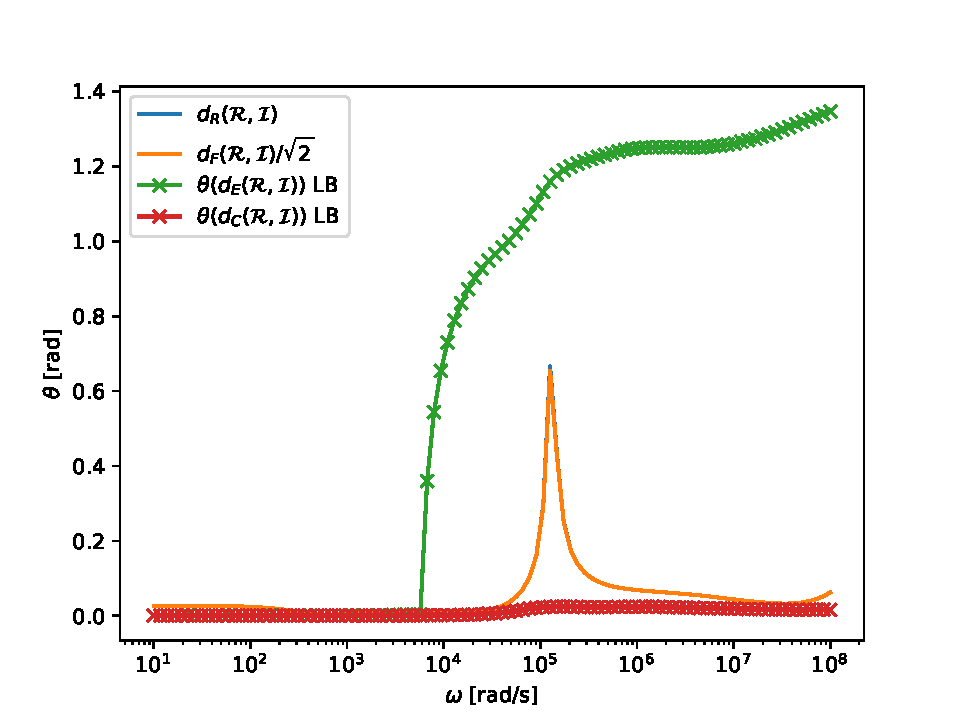
\includegraphics[width=0.3\textwidth]{mu40/OCC_Gun_modelv2_nonsym_StainSt_RI_al_0.01_40,1_sig_1e6,1e8_ord_4.pdf} \\
\lambda_i({\mathcal R}) &\lambda_i({\mathcal I}) &\text{Angles} \\ 
\end{array}$
\end{center}
\caption{Toy gun with $\mu_r=40$ in the barrel.  }
\end{figure}

\subsection{Barrel with $\mu_r=80$}

\begin{figure}[h]
\begin{center}
$\begin{array}{ccc}
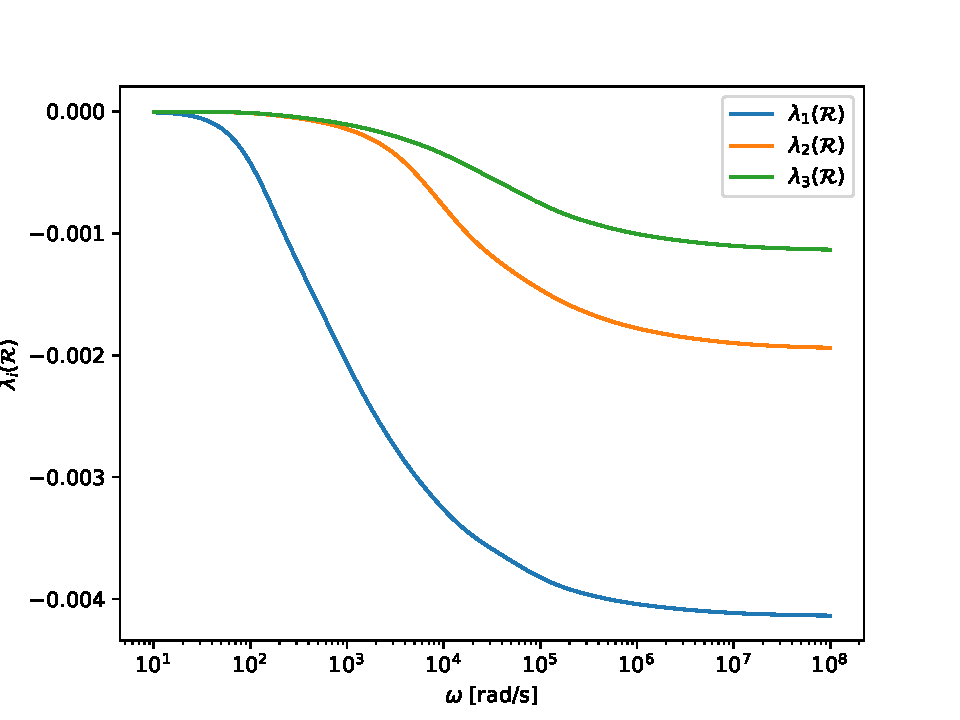
\includegraphics[width=0.3\textwidth]{mu80/OCC_Gun_modelv2_nonsym_StainSt_eig_R_al_0.01_80,1_sig_1e6,1e8_ord_5.pdf} &
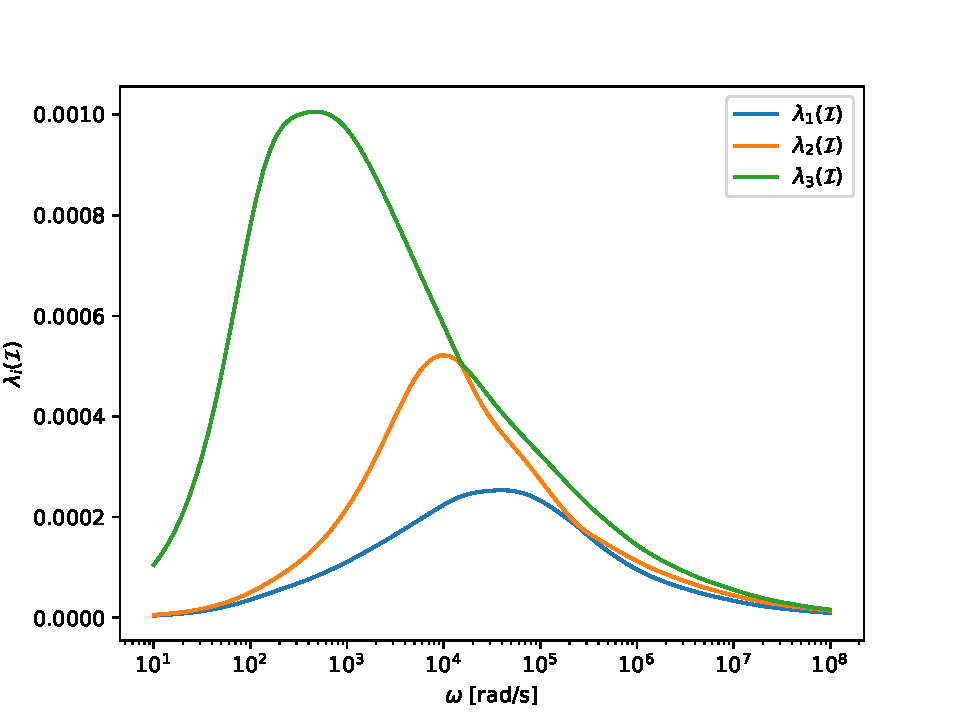
\includegraphics[width=0.3\textwidth]{mu80/OCC_Gun_modelv2_nonsym_StainSt_eig_I_al_0.01_80,1_sig_1e6,1e8_ord_5.pdf} &
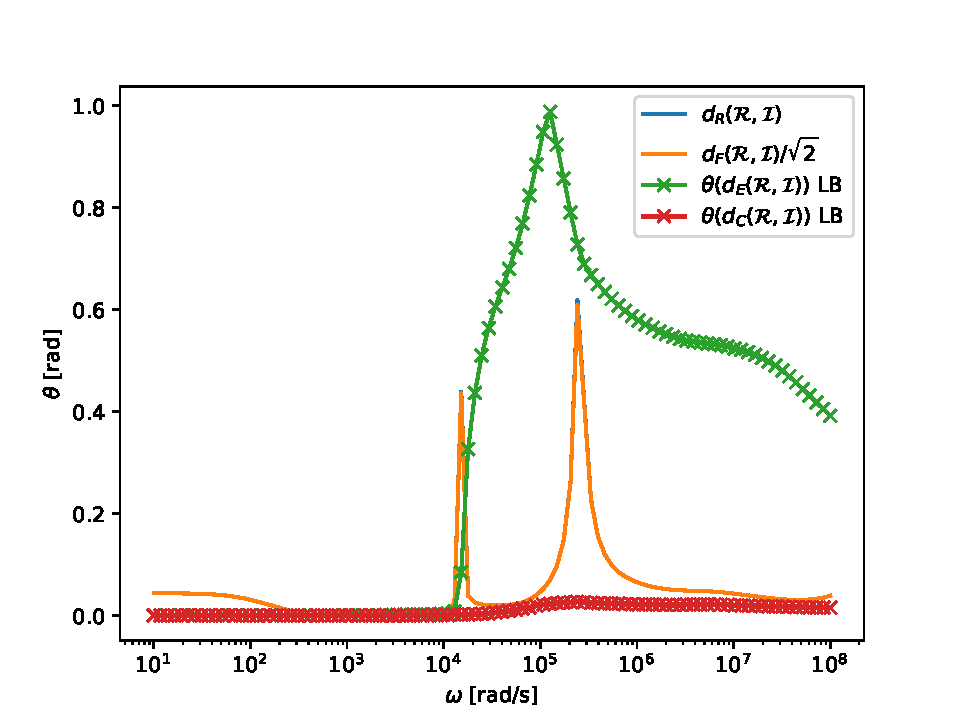
\includegraphics[width=0.3\textwidth]{mu80/OCC_Gun_modelv2_nonsym_StainSt_RI_al_0.01_80,1_sig_1e6,1e8_ord_5.pdf} \\
\lambda_i({\mathcal R}) &\lambda_i({\mathcal I}) &\text{Angles} \\ 
\end{array}$
\end{center}
\caption{Toy gun with $\mu_r=80$ in the barrel.  }
\end{figure}

\subsection{Barrel with $\mu_r=100$}

\begin{figure}[h]
\begin{center}
$\begin{array}{ccc}
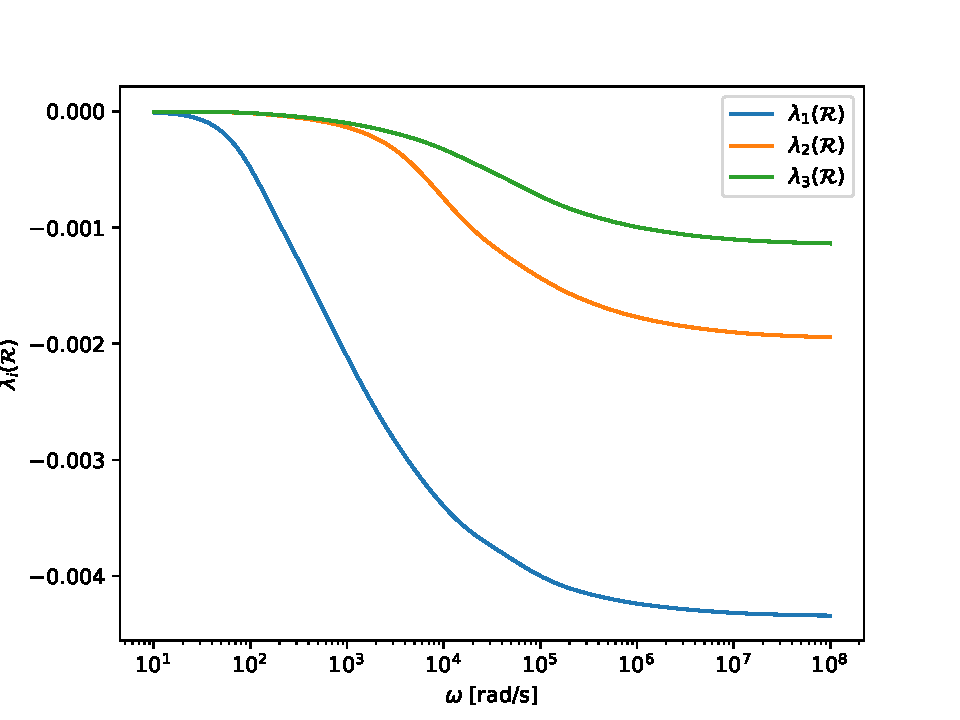
\includegraphics[width=0.3\textwidth]{mu100/OCC_Gun_modelv2_nonsym_StainSt_eig_R_al_0.01_100,1_sig_1e6,1e8_ord_5.pdf} &
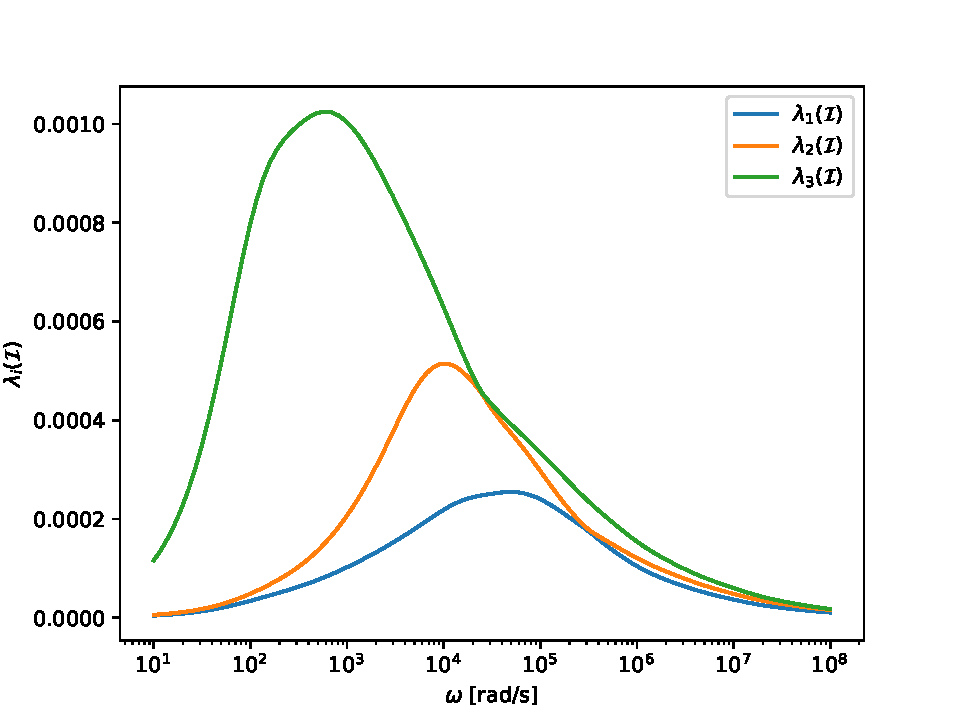
\includegraphics[width=0.3\textwidth]{mu100/OCC_Gun_modelv2_nonsym_StainSt_eig_I_al_0.01_100,1_sig_1e6,1e8_ord_5.pdf} &
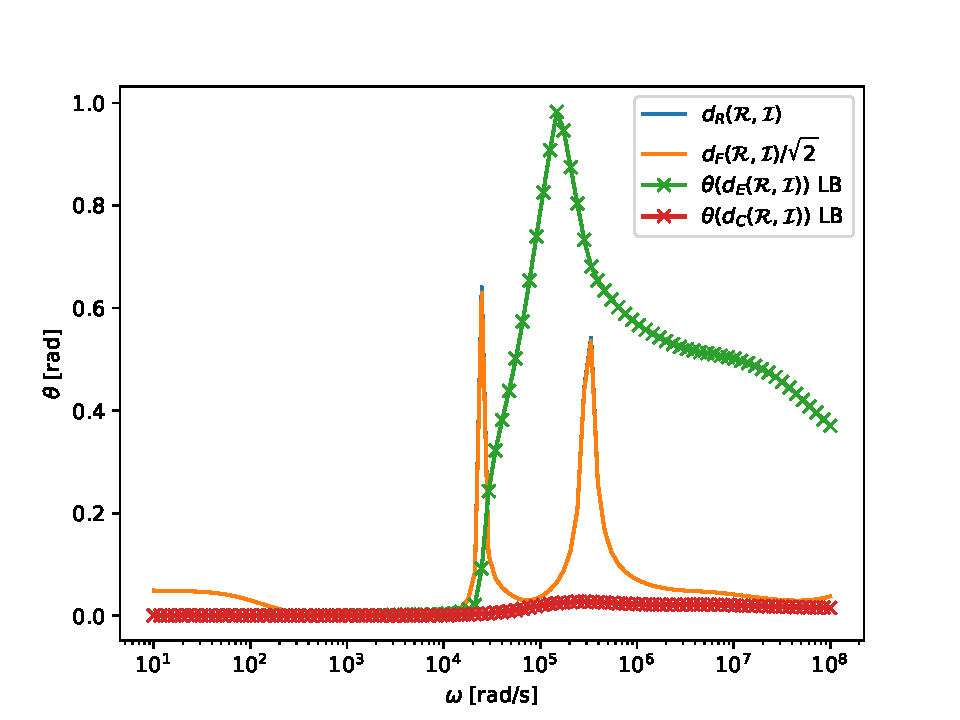
\includegraphics[width=0.3\textwidth]{mu100/OCC_Gun_modelv2_nonsym_StainSt_RI_al_0.01_100,1_sig_1e6,1e8_ord_5.pdf} \\
\lambda_i({\mathcal R}) &\lambda_i({\mathcal I}) &\text{Angles} \\ 
\end{array}$
\end{center}
\caption{Toy gun with $\mu_r=100$ in the barrel.  }
\end{figure}



\end{document}